\documentclass[a4paper]{article}   	
\usepackage{geometry} 
\usepackage[parfill]{parskip}    			% Activate to begin paragraphs with an empty line rather than an indent			
\usepackage{amsmath}		
\usepackage{amssymb}
\usepackage{dcolumn}
\usepackage{float}
\usepackage{enumitem}
\usepackage{titlesec}
\usepackage{subfiles}
\usepackage{tikz}	
\usepackage{graphicx}
\graphicspath{{plots/}}
							
\setlist{noitemsep} 					% no separation between list items
%\newcommand{\sectionbreak}{\clearpage}

%SetFonts

%SetFonts

%%%%%%%%%%%%%%%%%%%%%%%%%%%%%%%%%%%%%%%%%%%%%%%%%%%%%%%%%%%%%
% Preamble
%%%%%%%%%%%%%%%%%%%%%%%%%%%%%%%%%%%%%%%%%%%%%%%%%%%%%%%%%%%%%

\title{ECB Monetary Policy Spillovers to Middle Eastern and North African Countries}
\author{Carsten Stann}
\date{2019-10-07}	

%%%%%%%%%%%%%%%%%%%%%%%%%%%%%%%%%%%%%%%%%%%%%%%%%%%%%%%%%%%%%
% Begin Document
%%%%%%%%%%%%%%%%%%%%%%%%%%%%%%%%%%%%%%%%%%%%%%%%%%%%%%%%%%%%%

\begin{document}
\maketitle

%%%%%%%%%%%%%%%%%%%%%%%%%%%%%%%%%%%%%%%%%%%%%%%%%%%%%%%%%%%%%
% Introduction
%%%%%%%%%%%%%%%%%%%%%%%%%%%%%%%%%%%%%%%%%%%%%%%%%%%%%%%%%%%%%
\section{Introduction}

Using a simple pooled OLS panel regression model with dummy variables corresponding to ECB monetary policy announcements, this paper seeks to identify spillover effects to a series of financial variables in Middle East and North African (MENA) countries over the period 2008-01-03 to 2017-12-29.

Sample Countries
\begin{itemize}
   	\item Algeria, Bahrain, Egypt, Iraq, Israel, Jordan, Kuwait, Lebanon, Morocco, Oman, Qatar, Saudi Arabia, Syria, Tunisia, Turkey, United Arab Emirates, Yemen
\end{itemize}

Financial variables of interest
\begin{itemize}
	\setlength\itemsep{0em}
	\item Foreign Exchange Rates
	\item Stock Market Indices
	\item Interbank lending rates (3 months)
	\item Credit Default Swaps (5 year and 10 year maturities)
\end{itemize}
   
ECB Monetary Policy Programs
\begin{itemize}
	\item Liquidity providing
		\begin{itemize}
			\item long-term refinancing operations (LTRO)
			\item targeted longer-term refinancing operations (TLTRO)
		\end{itemize}
	\item Asset Purchases
		\begin{itemize}
			\item covered bond purchase program (CBPP1, CBPP2, CBPP3)
			\item securities markets program (SMP)
			\item outright monetary transactions (OMT)
			\item public sector purchase program (PSPP)
		\end{itemize}
	\end{itemize}
	
%%%%%%%%%%%%%%%%%%%%%%%%%%%%%%%%%%%%%%%%%%%%%%%%%%%%%%%%%%%%%
% Data
%%%%%%%%%%%%%%%%%%%%%%%%%%%%%%%%%%%%%%%%%%%%%%%%%%%%%%%%%%%%%
\section{Data}

All data was retrieved Reuters' Eikon database with the following codes:

% table of Eikon codes HERE

% exploratory plots
\begin{figure}[H]
	\centering
    	\caption{Financial Variables of Interest}
    	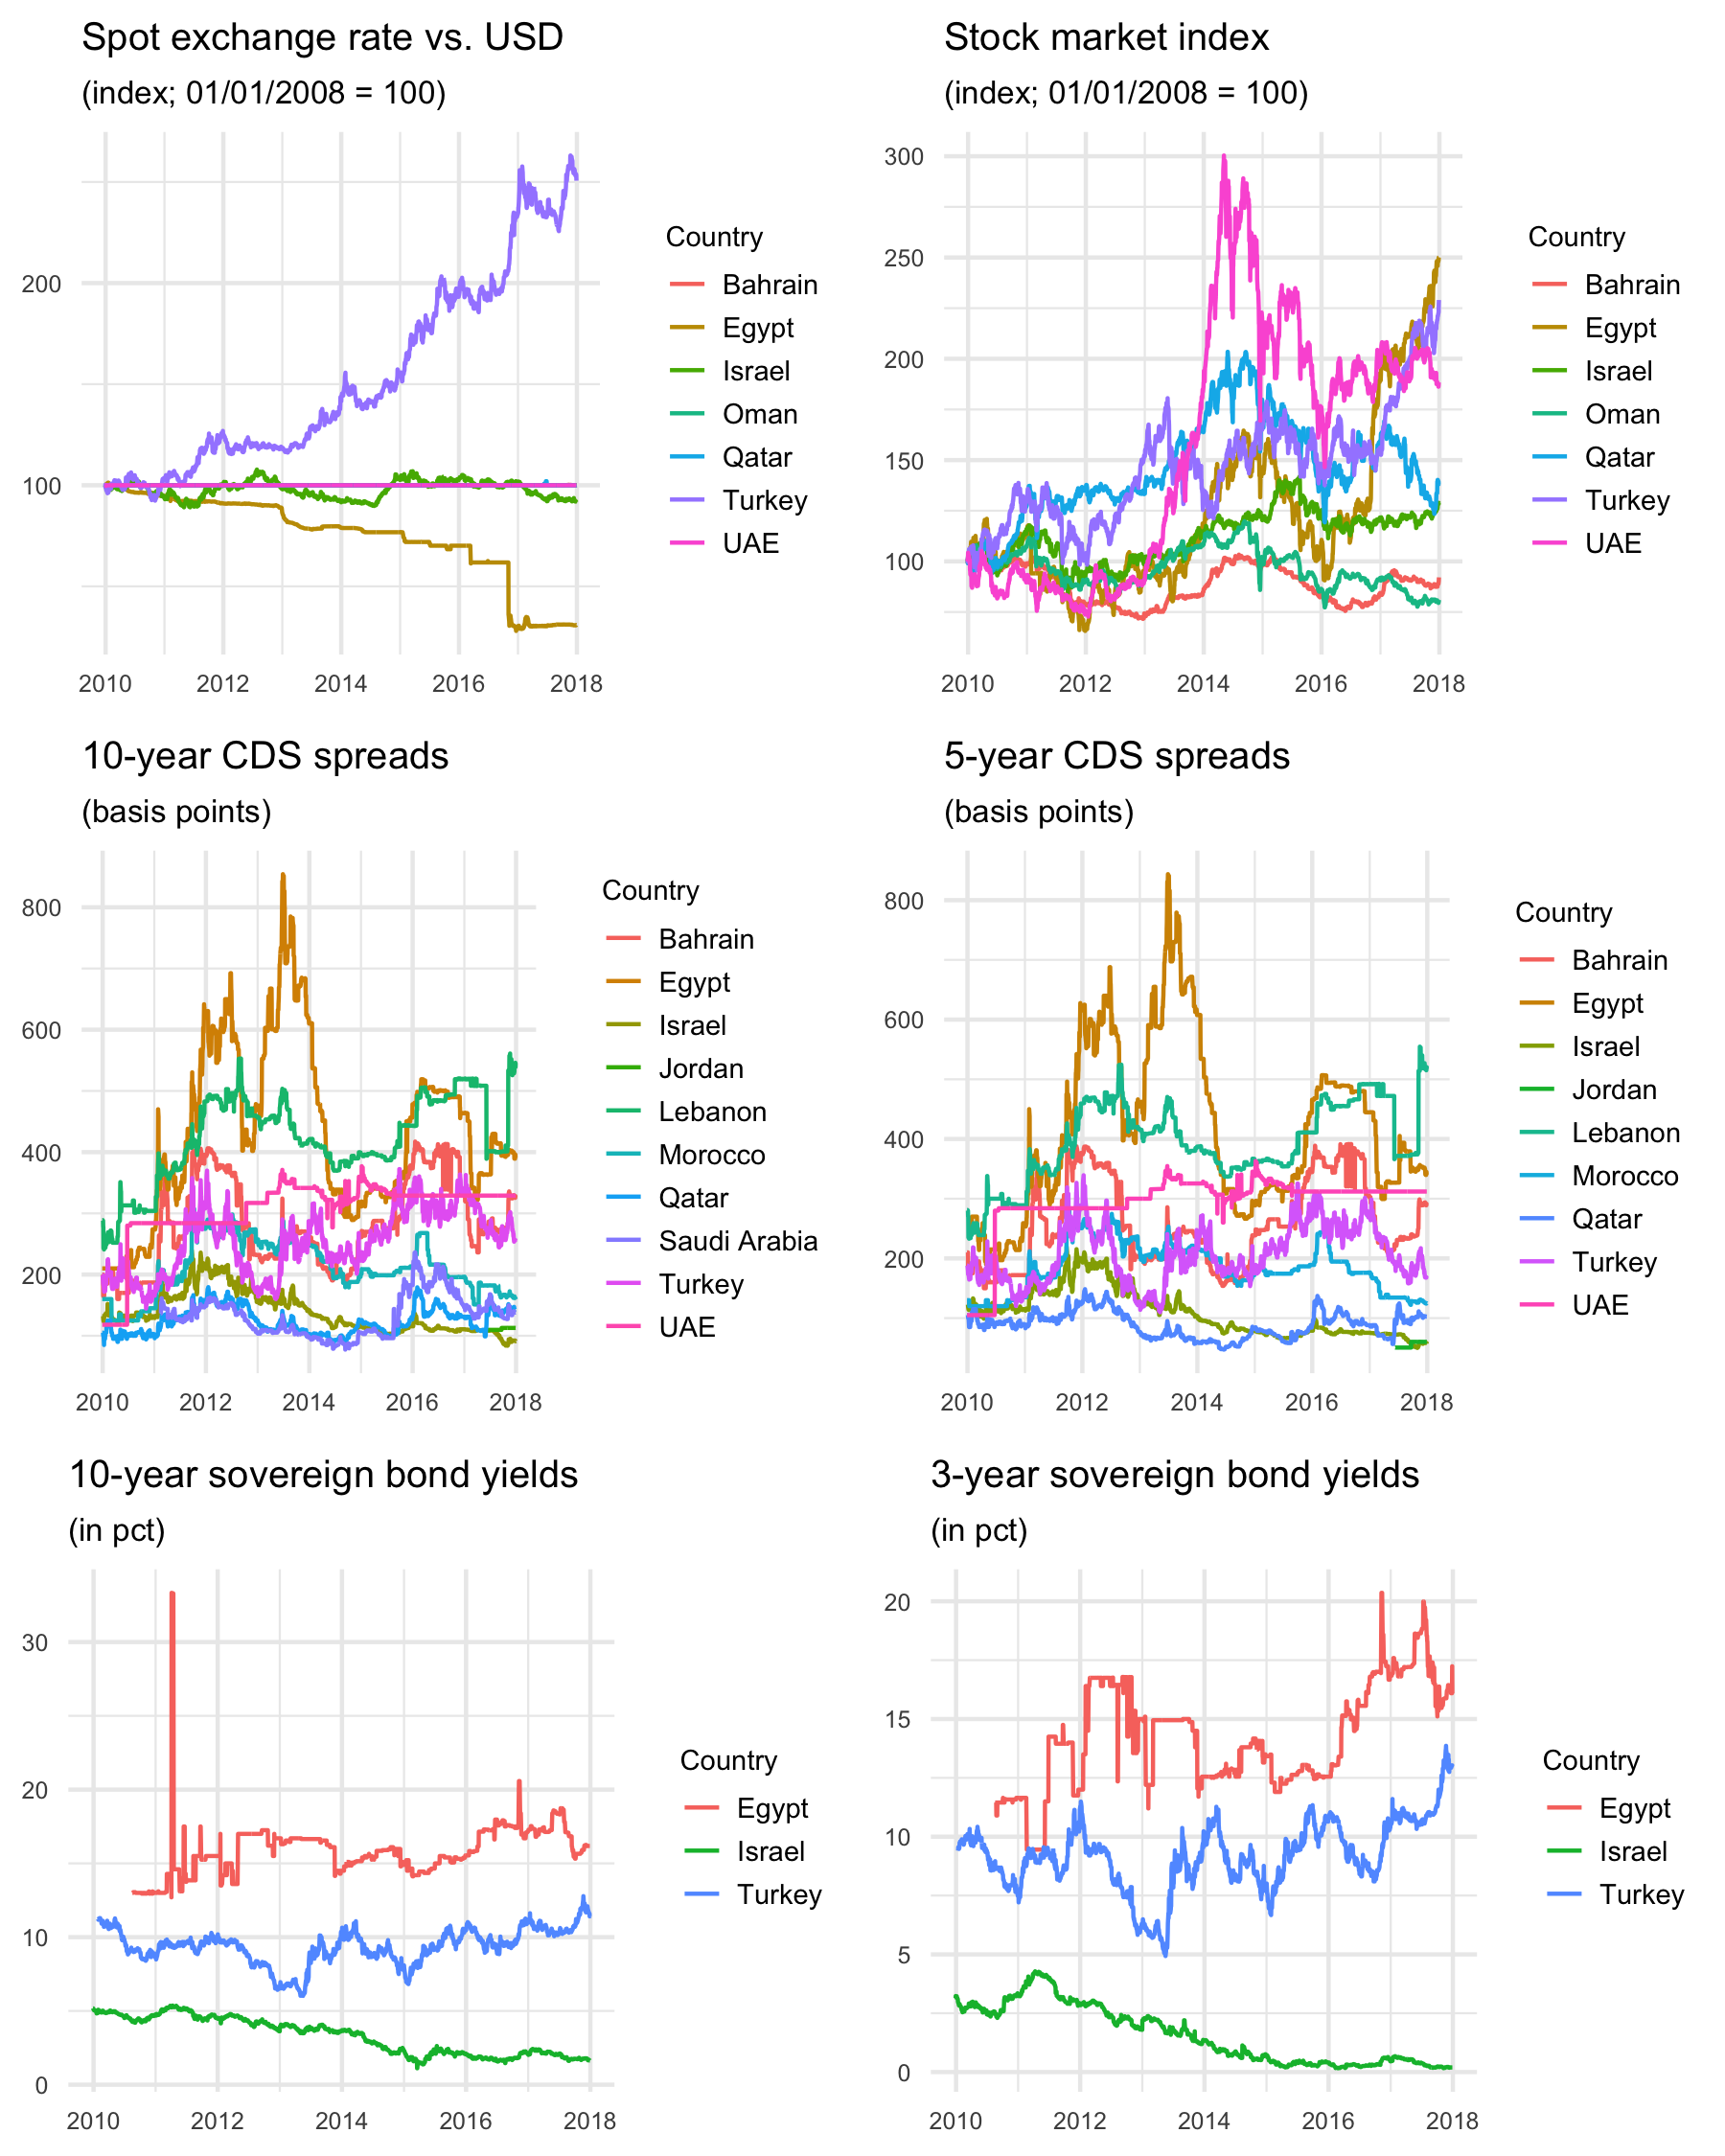
\includegraphics{input_data_plots}
	\label{figure:rawvars}
\end{figure}

\begin{figure}[H]
	\centering
	\caption{Foreign Exchange Rates}
	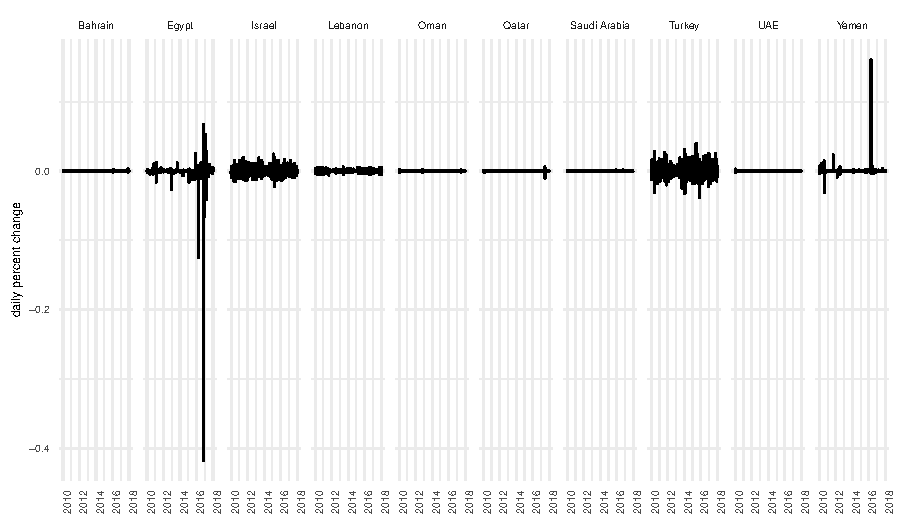
\includegraphics{fx_transformed}
	\label{figure:fxtransformed} 
\end{figure}

\begin{figure}[H]
	\centering
	\caption{Stock Market Indexes}
	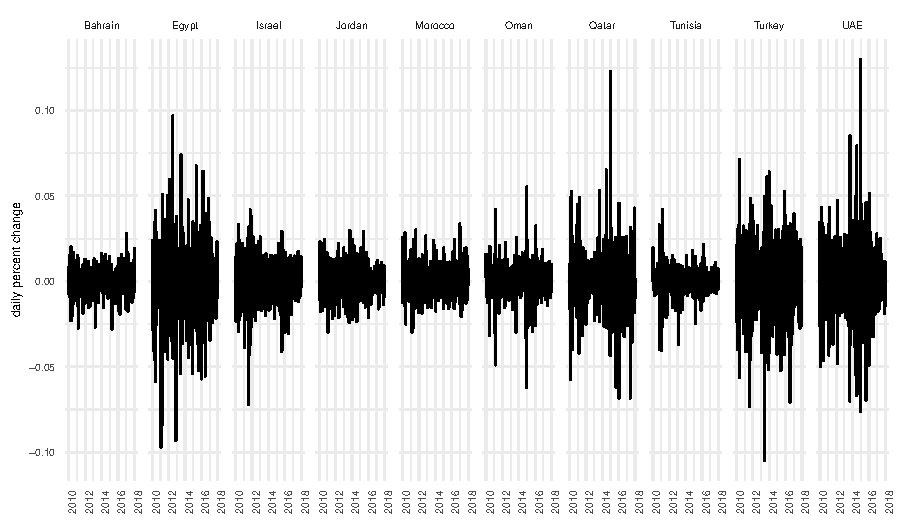
\includegraphics{stock_index_transformed}
	\label{figure:stocktransformed} 
\end{figure}

\begin{figure}[H]
	\centering
	\caption{Interbank Rates}
	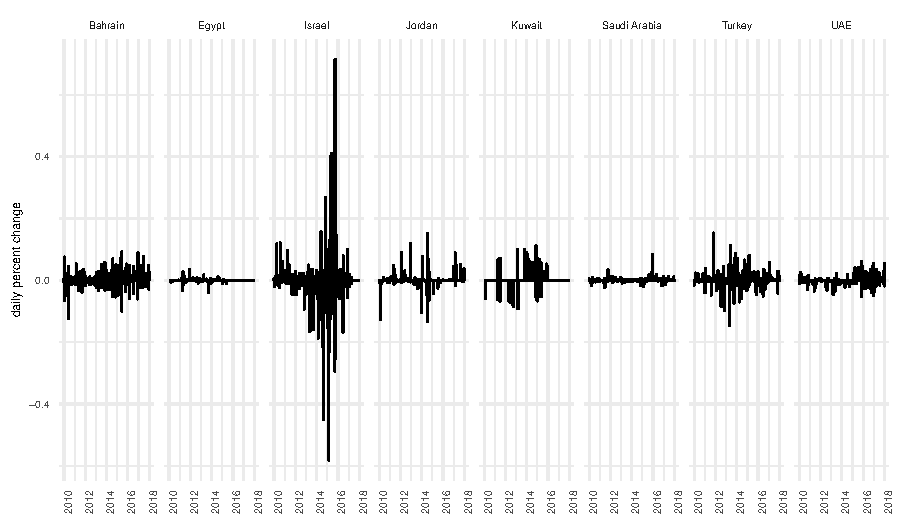
\includegraphics{interbank_transformed}
	\label{figure:interbanktransformed} 
\end{figure}

\begin{figure}[H]
	\centering
	\caption{Sovereign Bond Yields}
	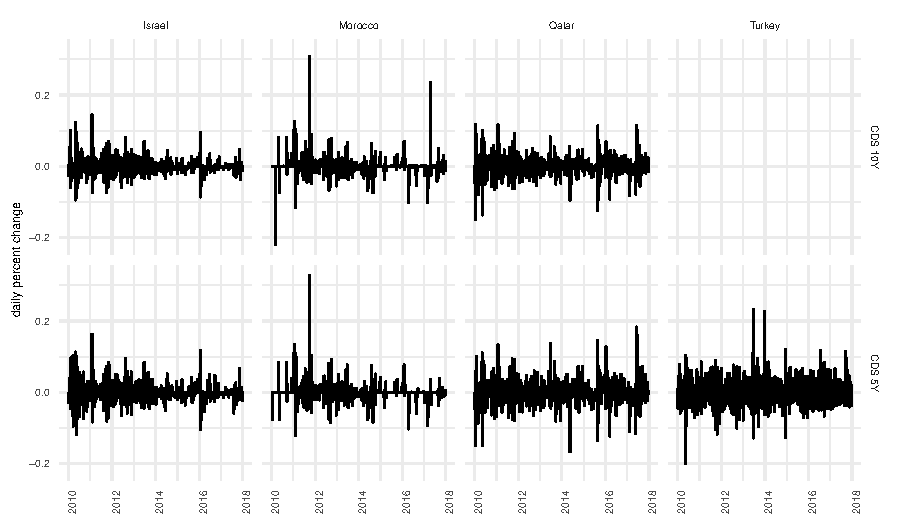
\includegraphics{cds_transformed}
	\label{figure:cdstransformed} 
\end{figure}

\begin{figure}[H]
	\centering
	\caption{Sovereign Bond Yields}
	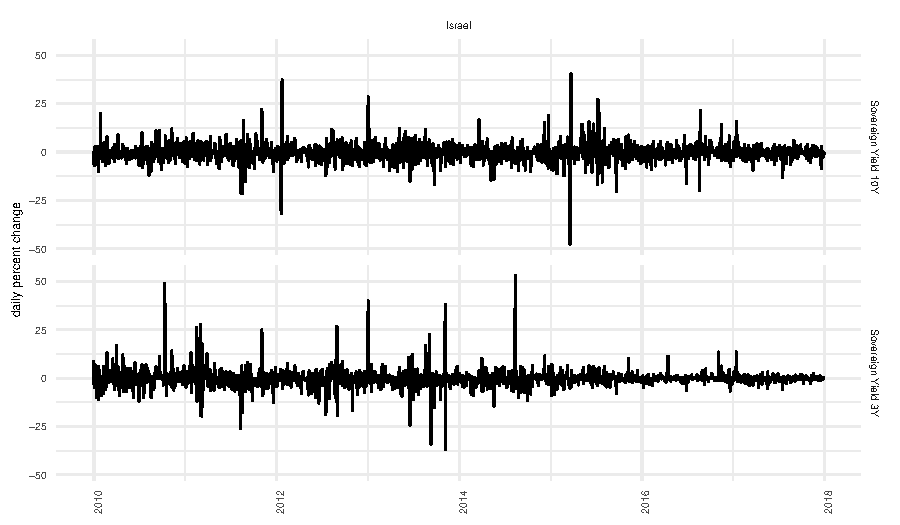
\includegraphics{sovereign_yield_transformed}
	\label{figure:sovereignstransformed} 
\end{figure}

\subsection{Missingness}

The largest challenge in conducting this analysis is data availability. The use of monetary policy announcement dummy variables on a 1-day window requires daily data for all financial variables of interest. For many countries, only a subset of the financial variables of interest are fully available for the full sample period (2008-01-03 to 2017-12-29). The following chart shows the "missingness" of each variable across all MENA countries.In order to maintain fully balanced panel data samples, only series with no missing values on the sample period were selected for the regressions.

\begin{figure}[H]
	\centering
	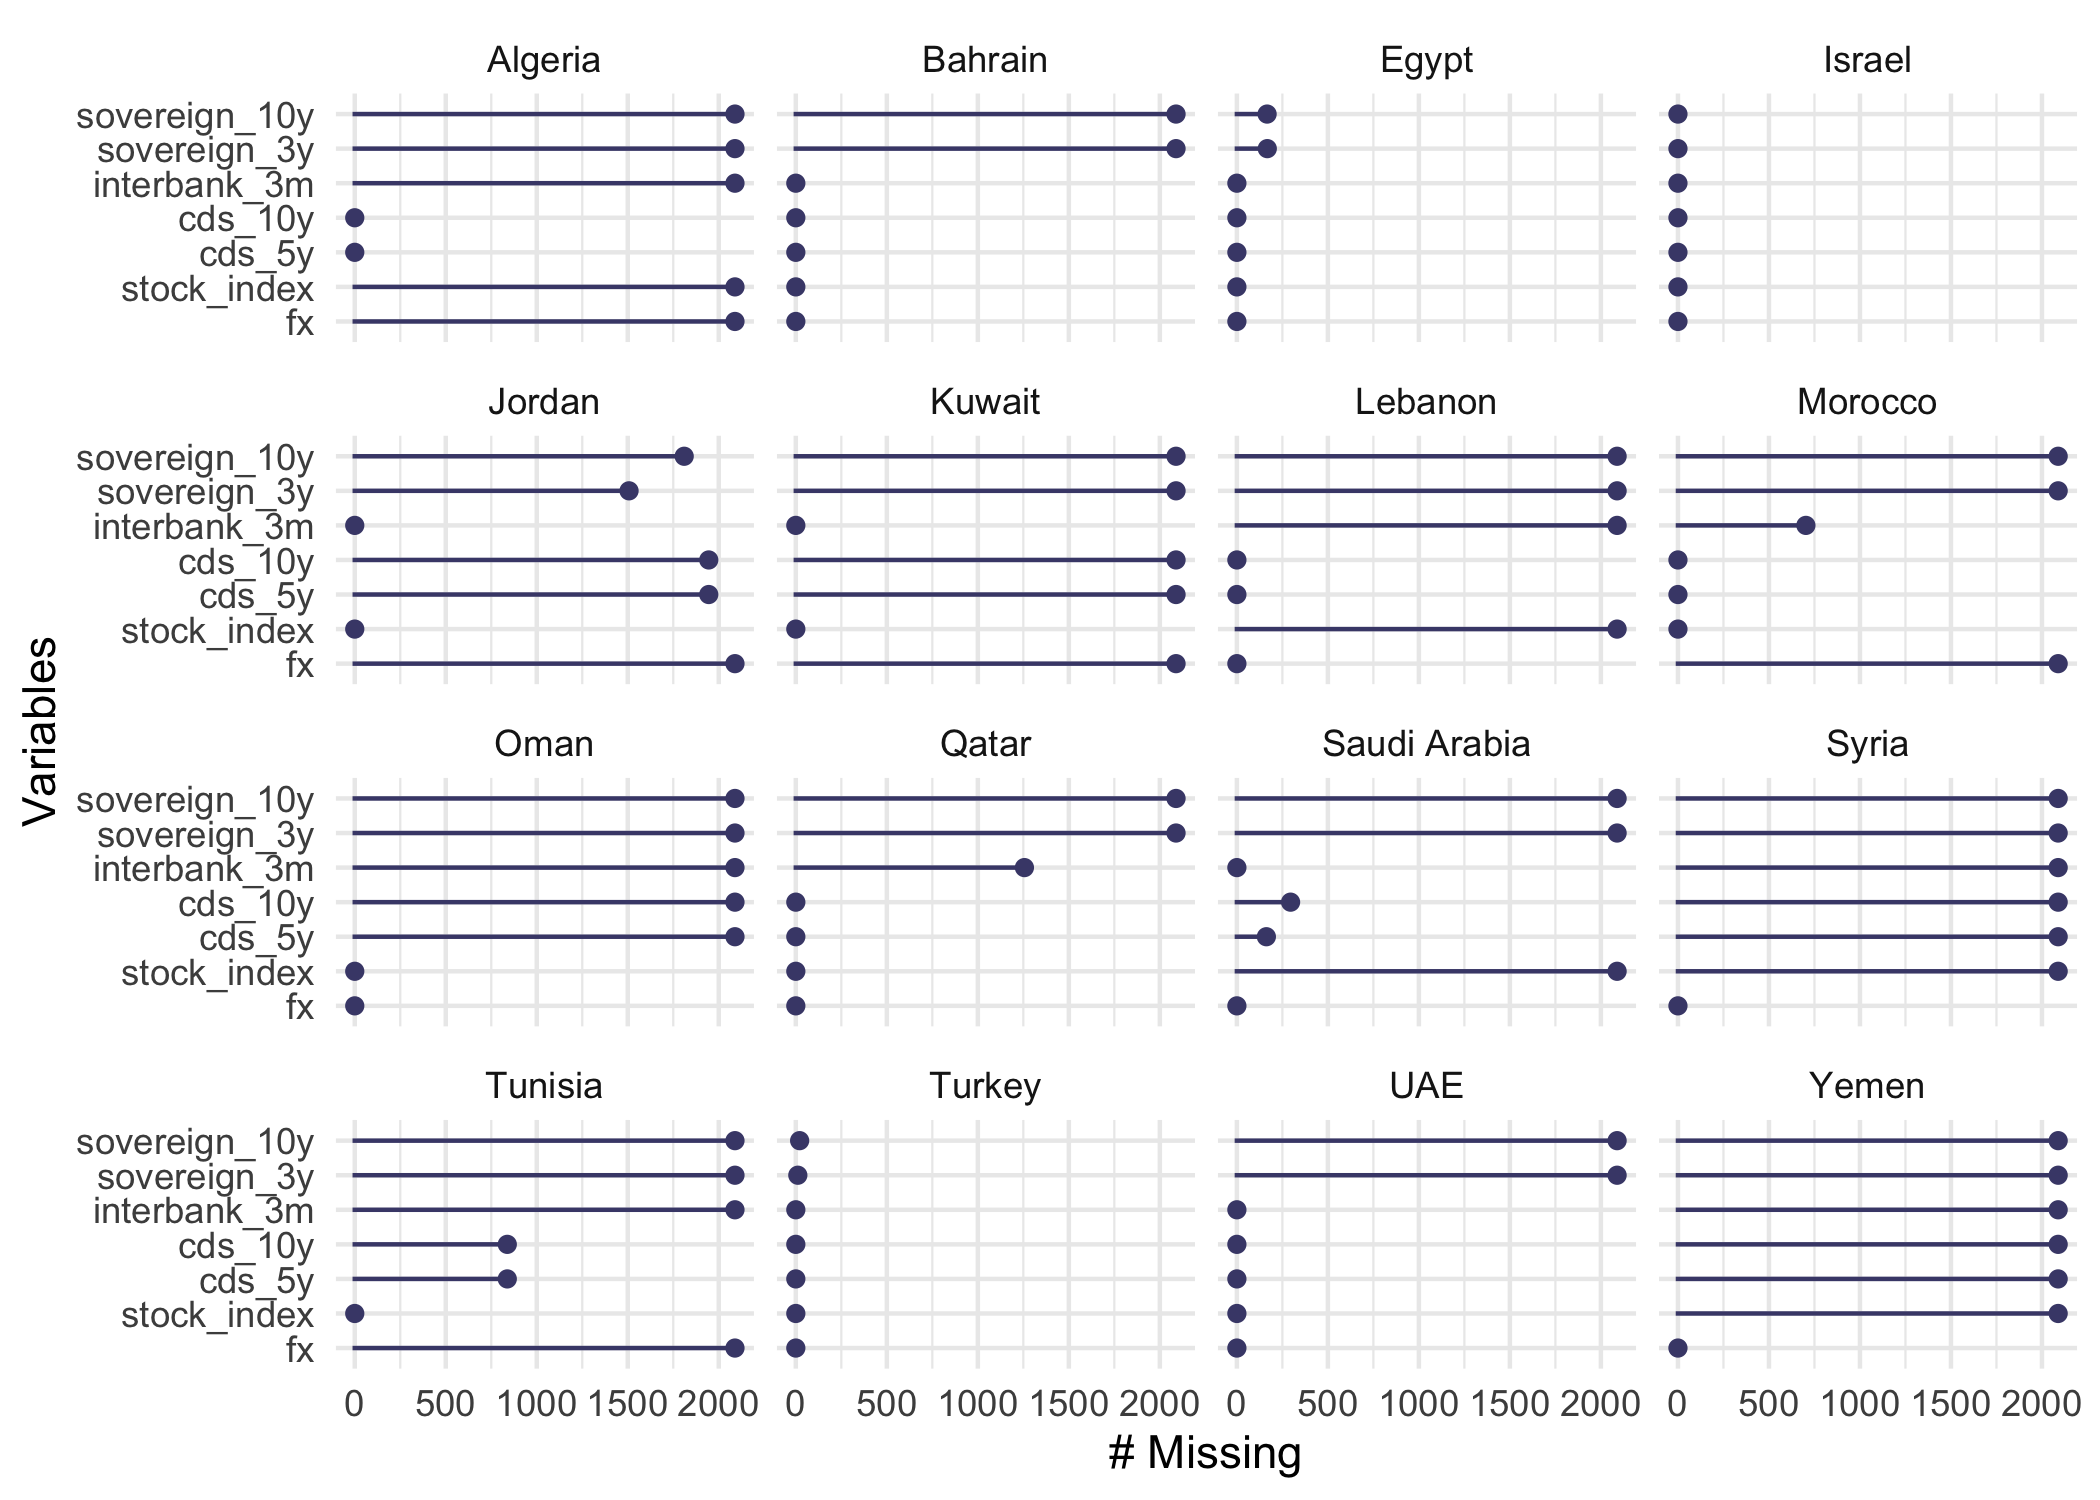
\includegraphics{missingness}
	\caption{Missing Values in Data by Country and Series}
	\label{figure:missingness} 
\end{figure}



% Table of missing values here
	
%%%%%%%%%%%%%%%%%%%%%%%%%%%%%%%%%%%%%%%%%%%%%%%%%%%%%%%%%%%%%
% Empirical Approach
%%%%%%%%%%%%%%%%%%%%%%%%%%%%%%%%%%%%%%%%%%%%%%%%%%%%%%%%%%%%%
\section{Empirical Approach}

\subsection{Linear Panel Model}

The general form of a pooled OLS model can be described through the following specification:

$$y_{it} = \alpha + x_{it}\beta + \epsilon_{it}$$

where $i=1,...,n$ indexes individual countires, $t=1,...,T$ is the time index, and $\epsilon_{it}$ is a random disturbance term. The key element of this approach is paramener homogeneity, meaning that the constant $\alpha$ and the estimated coeffcient $\beta$ terms follow $\alpha_{it} = \alpha$ and $\beta_{it} = \beta$ for all $i,t$. 

Following the general form specified above, this analysis employs the following regression: 

$$\Delta y_{i,t} = \alpha + \beta_1 MP^{ECB}_t + \beta_2 \Delta IR^{ECB}_t + \beta_3 \Delta VIX_t + \beta_4 y_{i,t-1} + \epsilon_{i,t}$$

where $y_{i,t}$ represents the financial variable of interest, $MP^{ECB}_t$ a vector of monetary policy dummy variables, $IR^{ECB}_t$ the rate on the ECB;s marginal lending facility, and $VIX_t$ a volatility index used to control for periods of high volatility in financial markets that may otherwise have falsely attributed spillovers to announcements. 

The financial variables of interest were transformed along the following specification:

\begin{itemize}
	\item Daily change in bps: 
		\begin{itemize}
			\item interbank lending rate
			\item ECB marginal lending rate
		\end{itemize}
	\item Daily discrete rate of changes: 
		\begin{itemize}
			\item exchange rates
			\item stock market indices
			\item volatility index
			\item credit default swaps
		\end {itemize}
\end{itemize}



%%%%%%%%%%%%%%%%%%%%%%%%%%%%%%%%%%%%%%%%%%%%%%%%%%%%%%%%%%%%%
% Results
%%%%%%%%%%%%%%%%%%%%%%%%%%%%%%%%%%%%%%%%%%%%%%%%%%%%%%%%%%%%%
\section{Results}

A panel regression was estimated for each financial variable of interest. Due to data availability, each regression contains only a subset of all MENA countries. The following table indicates which countries were included in each regression.

% Panel regression output here

\subfile{tables/plm_liquidity.tex}

\subfile{tables/plm_purchases.tex}

\subfile{tables/plm_smp.tex}

\subfile{tables/plm_omt.tex}

\subfile{tables/plm_PSPP.tex}

\subfile{tables/plm_cbpp.tex}

\subfile{tables/plm_abspp.tex}

\subfile{tables/plm_cspp.tex}


\end{document}  